\documentclass[a4paper, 12pt]{article}

% \usepackage[portuges]{babel}
\usepackage[utf8]{inputenc}
\usepackage{amsmath,amssymb}
\usepackage{graphicx}
\usepackage{subcaption}
\usepackage[colorinlistoftodos]{todonotes}

\usepackage{indentfirst}
\usepackage{verbatim}
\usepackage{textcomp}
\usepackage{gensymb}
\usepackage{tikz-feynman}
\usepackage{wrapfig}
\usepackage{physics}

\usepackage{relsize}

\usepackage{lipsum}% http://ctan.org/pkg/lipsum
\usepackage{xcolor}% http://ctan.org/pkg/xcolor
\usepackage{xparse}% http://ctan.org/pkg/xparse
\NewDocumentCommand{\myrule}{O{1pt} O{2pt} O{black}}{%
  \par\nobreak % don't break a page here
  \kern\the\prevdepth % don't take into account the depth of the preceding line
  \kern#2 % space before the rule
  {\color{#3}\hrule height #1 width\hsize} % the rule
  \kern#2 % space after the rule
  \nointerlineskip % no additional space after the rule
}
\usepackage[section]{placeins}

\usepackage{booktabs}
\usepackage{colortbl}%
   \newcommand{\myrowcolour}{\rowcolor[gray]{0.925}}
   
\usepackage[obeyspaces]{url}
\usepackage{etoolbox}
\usepackage[colorlinks,citecolor=black,urlcolor=blue,bookmarks=false,hypertexnames=true]{hyperref} 

\usepackage{geometry}
\geometry{
	paper=a4paper, % Change to letterpaper for US letter
	inner=3cm, % Inner margin
	outer=3cm, % Outer margin
	bindingoffset=.5cm, % Binding offset
	top=2cm, % Top margin
	bottom=2cm, % Bottom margin
	%showframe, % Uncomment to show how the type block is set on the page
}
%*******************************************************************************%
%************************************START**************************************%
%*******************************************************************************%
\begin{document}

%************************************TITLE PAGE**************************************%
\begin{titlepage}
	\begin{center}
	\textbf{\LARGE Nankai University}\\[0.5cm] 
	\textbf{\large School of Physics, Boling Class}\\[0.2cm]
	\vspace{20pt}
	\par
	\vspace{20pt}
	\textbf{\Large 2023 Summer \quad \quad Sapienza Università di Roma}\\
	\vspace{15pt}
	\myrule[1pt][7pt]
	\textbf{\LARGE A Fundemental Study on Photon Isolation}\\
	\vspace{15pt}
	\textbf{\large Summer Research Report}\\
	\myrule[1pt][7pt]
	\vspace{25pt}
	\textbf{\large Song Xianglong \hspace{20pt} Prof. Leticia Cunqueiro}\\

	\end{center}
\end{titlepage}
\newpage

\tableofcontents
\phantom{0}\\
\phantom{0}\\
\phantom{0}\\
\phantom{0}\\
\phantom{0}\\


\section{Introduction}
	In Quantum Electrodynamics (QED), splitting refers to a process where a high-energy particle emits or dacays a daughter 
	particle and undergoes a change in its state. This process is governed by the principles of QED, which is the quantum 
	field theory describing the electromagnetic force.\par
	\begin{wrapfigure}{l}{0.6\textwidth}
		\centering
		\begin{tikzpicture}
			\begin{feynman}
				\vertex (a) {\(q\)};
				\vertex [right=of a] (b) ;
				\vertex [above right=of b] (f1) {\(\gamma\)};
				\vertex [below right=of b] (c) {\(q\)};
				\diagram* {
				  (a) -- [fermion] (b) -- [photon] (f1),
				  (b) -- [fermion] (c),
				};
			  \end{feynman}
		\end{tikzpicture}
		\caption{Feynman diagram for \(q \rightarrow q\gamma\).}
		\label {fig:feynman}
	\end{wrapfigure}
	Here we are interested in  $q\rightarrow q\gamma$ process (Fig. 1). Which refers to the quark undergoing a transition where it
	emits a photon. The emission of a photon by a quark can occur in various high-energy processes, and it contributes to the
	dynamics of particle interactions in experiments such as those conducted at particle colliders.\par
	The probability for a quark to radiate a photon with some angle $\theta_{\gamma}$ and momentum fraction $z_{\gamma}$ is given by:
	\begin{equation}
		\dd P_{q\rightarrow q\gamma}=\frac{\alpha_ee^2}{2\pi}\frac{\dd \theta_{\gamma}}{\theta_{\gamma}}P(z_{\gamma})\dd z_{\gamma},\quad
		P(z)=\left(\frac{1+(1-z)^2}{z}\right)_+,
	\end{equation}
	where $P(z)$ is the (regularized) QED splitting function \cite{hall2018photon}. The QED splitting function gives the probability
	density for a quark to emit a photon with a certain fraction of its energy. The quark can lose energy by emitting a photon, and the
	splitting function characterizes the likelihood of this energy loss. The form of the QED splitting function depends on the specific
	process under consideration and is derived using perturbation theory. QED splitting function plays an important role in high 
	energy experiments thus we put a great emphasis on it. In this study, we use soft drop isolation to explore the QED splitting function
	in $q\rightarrow q\gamma$ process.


\section{Grooming}
	Jet grooming refers to a set of techniques used to improve the reconstruction and analysis of jets. Jets can be affected by various
	effects, such as soft radiation and pileup, which can lead to a broader or less well-defined jet structure. Grooming methods help
	mitigate these effects and enhance the precision of jet measurements.\par
	Soft radiation, characterized by low momentum particles, can significantly impact the structure of jets, making them broader and
	less well-defined. Grooming techniques, such as trimming, pruning, and soft drop, are designed to remove soft radiation from jets,
	providing a more accurate measurement of the core jet properties. And grooming methods improve the discrimination between jets
	originating from hard-scattering processes (signal) and those influenced by soft radiation or pileup (background). By removing
	wide-angle and soft radiation components, grooming helps to enhance the purity of the signal sample, making it easier to identify.
	Also, different experimental conditions, such as varying center-of-mass energies and detector configurations, can impact the
	performance of jet algorithms. Grooming methods provide a way to adapt to these conditions, improving the robustness and consistency
	of jet measurements across different experimental setups.\par
	Grooming is widely used in experiments at high-energy colliders like the Large Hadron Collider (LHC) at CERN, where the production
	of jets is abundant.\par
	\subsection{Soft Drop Algorithm}
		Soft Drop is a grooming algorithm that involves recursively declustering a jet into two subjets and rejecting the subjet with the
		lower momentum if certain conditions are not met. It is designed to be sensitive to both soft radiation and wide-angle radiation.\par
		Soft drop declustering is used to identify hard subjets within a jet that satisfy the condition:
		\begin{equation}
			\frac{\min(p_{T1},p_{T2})}{p_{T1}+p_{T2}}\geq z_{\mathrm{cut}}\left(\frac{R_{12}}{R_0}\right)^{\beta},
		\end{equation}
		where $p_{Ti}$ are the transverse momenta of the subjets, $R_{12}$ is their pairwise angular separation, $R_0$ is the jet radius
		parameter, and $z_{\mathrm{cut}}$ and $\beta$ are the parameters of the soft drop algorithm. The two parameters control the sensitivity of
		the Soft Drop algorithm to soft radiation and wide-angle radiation. A smaller $z_{\mathrm{cut}}$ enhances the removal of soft radiation, while
		$\beta$ controls the angular scaling.\par
		Soft drop isolation is a method derives from soft drop declustering and it inverts the condition of soft drop declustering,
		thereby selecting “photon jets” with no appreciable substructure.


\section{Photon Isolation}
	\subsection{Procedure}
		The photon isolation procedure is a combination of soft drop declustering and soft drop isolation.\par
		First we start with a jet with radius $R=0.4$ which is obtained by ankt-$k_T$ algorithm. Then first we apply soft drop declustering
		with $z_{\mathrm{cut}}=0.1$, $\beta=0$, $R_0=R=0.4$ to the jet. Thus we have two prongs and then it comes to soft drop isolation.\par
		For soft drop isolation, we set $z_{\mathrm{cut}}=0.1$, $\beta=2$, $R_0=R_{12}/2$. Only if we go through all the declustering and
		we don't find a splitting that passes the cut and at the same time the last particle in the declustering is a photon, we regard
		it as an isolated photon subjet.
	\subsection{Some Observables}
		\subsubsection{$z_{\mathrm{iso}}$}
			The QED splitting function describes the probability distribution of the momentum sharing $z$ between the photon and the
			quark. We define the isolated photon momentum sharing as
			\begin{equation}
				z_{\mathrm{iso}}=\frac{p_{T\gamma-\mathrm{sub}}}{p_{T\gamma-\mathrm{sub}}+p_{T\mathrm{had}-\mathrm{sub}}}.
			\end{equation}
			Where $p_{T\gamma-\mathrm{sub}}$ is the transverse momentum of the isolated photon subjet and $p_{T\mathrm{had}-\mathrm{sub}}$
			is the transverse momentum of the other (hadronic) subjet.
		\subsubsection{$\theta$}
			$\theta$ denotes the angular distance between two objects in the $\eta-\phi$ plane, where $\eta$ is the pseudorapidity
			and $\phi$ is the azimuthal angle. For the two subjets in soft drop,
			\begin{equation}
				\Delta R_{12}=\sqrt{(\Delta \eta)^2+(\Delta \phi)^2}.
			\end{equation}
			For the soft drop algorithm, after each declustering step, the angular separation $\Delta R_{12}$ between the two
			subjets is calculated, and this separation is used in the soft drop condition. The condition ensures that the soft
			radiation and wide-angle radiation within the jet are treated appropriately.\par
			The $\Delta R_{12}$ term in the denominator is normalized by the jet radius $R$ to make it dimensionless and is raised
			to the power of $\beta$ to control the angular scaling. The soft drop condition ensures that the softer subjet is not
			too collinear with the harder subjet, effectively removing soft radiation from the jet.


\section{Parton Shower Study}
	We perform a parton shower study in \textsc{Pythia} 8.309 \cite{Sj_strand_2006} \cite{Sj_strand_2015} and generate 100 million
	events from proton-proton collisions. Jet clustering and photon isolation were performed using \textsc{FastJet} 3.4.1 \cite{Cacciari_2012}.\par
	We firt make a brief introduction to \textsc{Pythia} and \textsc{FastJet}, and then we discuss the result.
	\subsection{Pythia}
		\textsc{Pythia} is a program for the generation of high-energy physics collision events, i.e. for the description of collisions at
		high energies between electrons, protons, photons and heavy nuclei. It contains theory and models for a number of physics
		aspects, including hard and soft interactions, parton distributions, initial- and final-state parton showers, multiparton
		interactions, fragmentation and decay. It is largely based on original research, but also borrows many formulae and other
		knowledge from the literature. As such it is categorized as a general purpose Monte Carlo event generator.
	\subsection{FastJet}
		\textsc{FastJet} is a software package for jet finding in $pp$ and $e^+e^-$ collisions. It includes fast native implementations
		of many sequential recombination clustering algorithms, plugins for access to a range of cone jet finders and tools for advanced
		jet manipulation. It provides a fast implementation of several longitudinally invariant sequential recombination jet algorithms, in
		particular the longitudinally invariant kt jet algorithm, the inclusive longitudinally invariant version of the Cambridge/Aachen
		jet-algorithm, and the inclusive anti-kt algorithm.
	\subsection{Result}
		For event selection, we require $p_{T\mathrm{jet}}>350\mathrm{~GeV}$ as a defult setting.
		\begin{figure}[t]
			\centering
			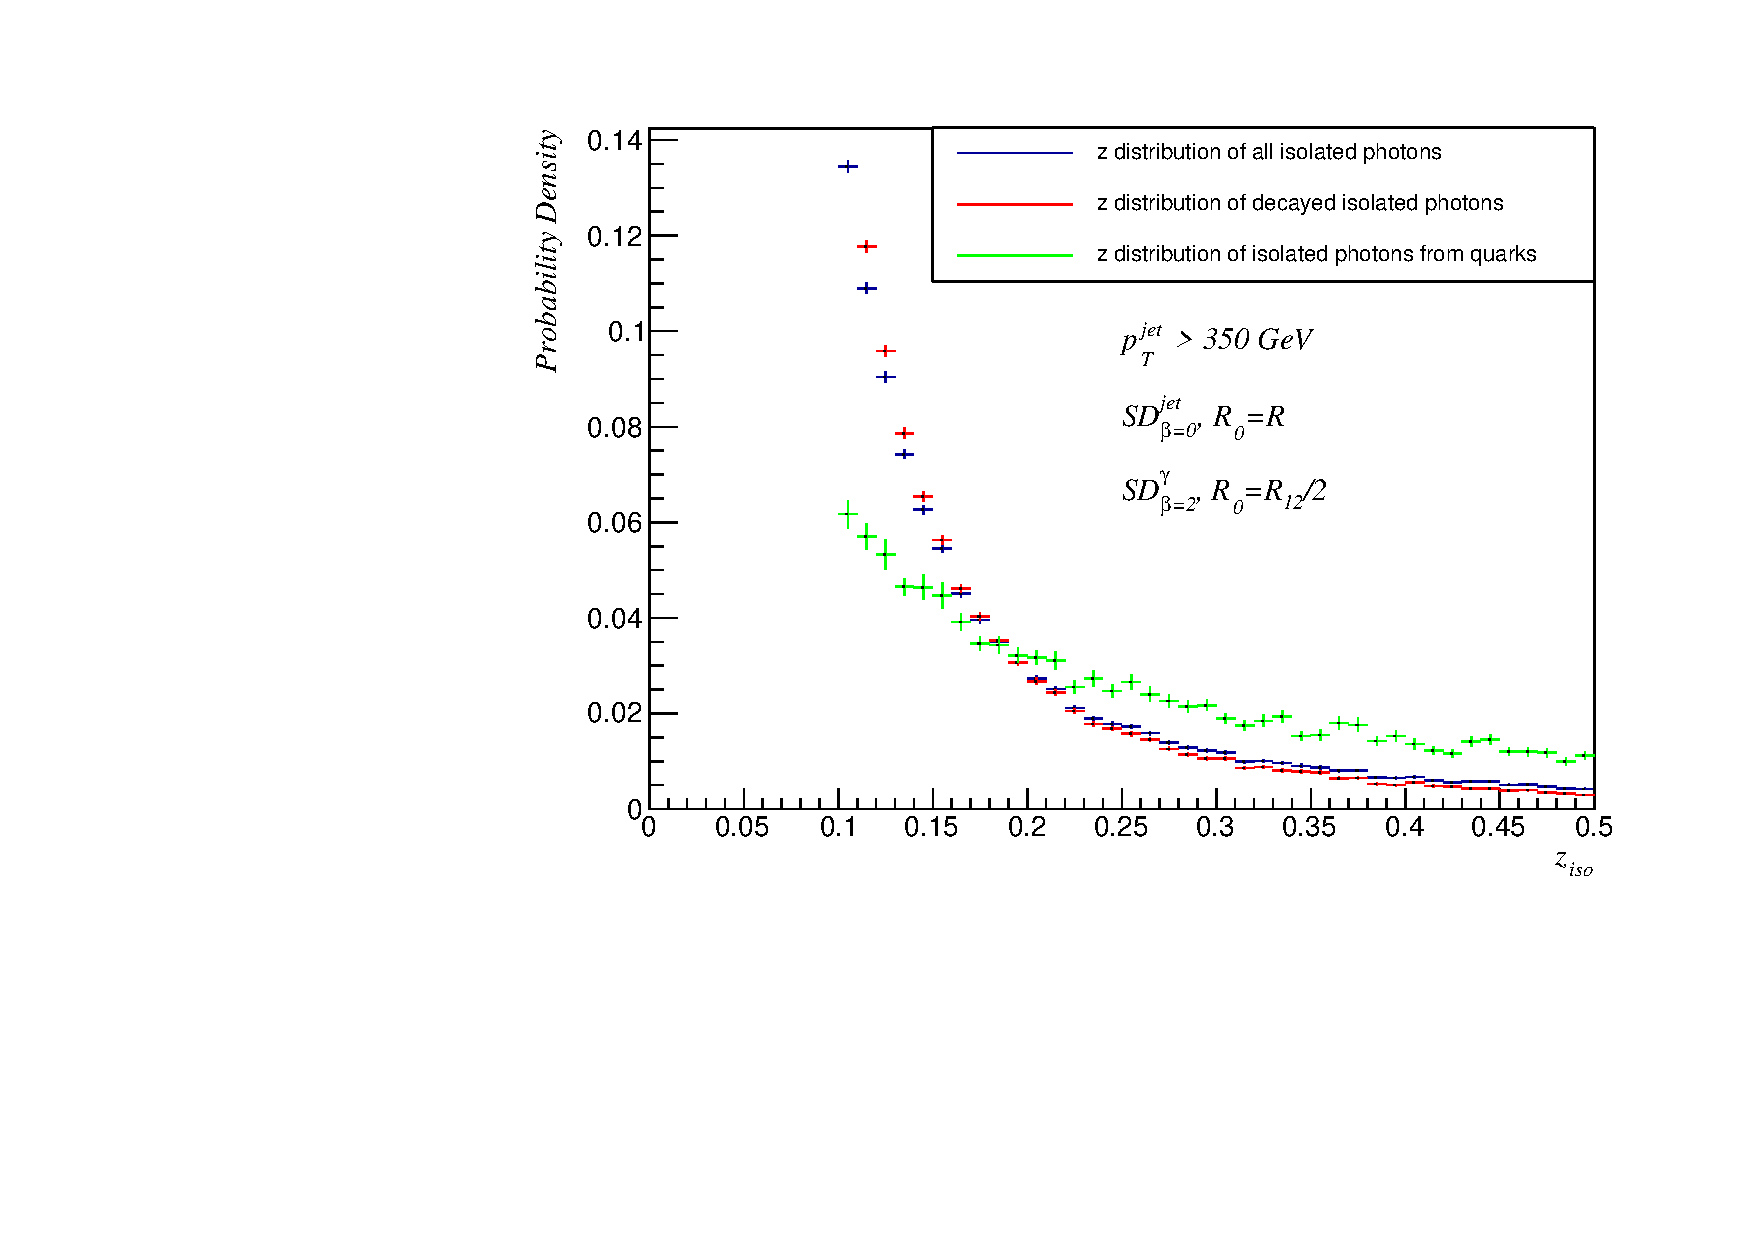
\includegraphics[width=\linewidth]{1.pdf}
			\caption{All isolated photons without $\theta_{\mathrm{cut}}$}
		\end{figure}
		In Fig. 2, we show the $z$ distribution of all isolated photons ($p_{T\mathrm{jet}}>350\mathrm{~GeV}$), which is, including
		photons from quarks and photons from measons' ($\eta$ and $\pi_0$) decay.\par
		\begin{figure}[t]
			\centering
			\begin{subfigure}{0.47\linewidth}
				\centering
				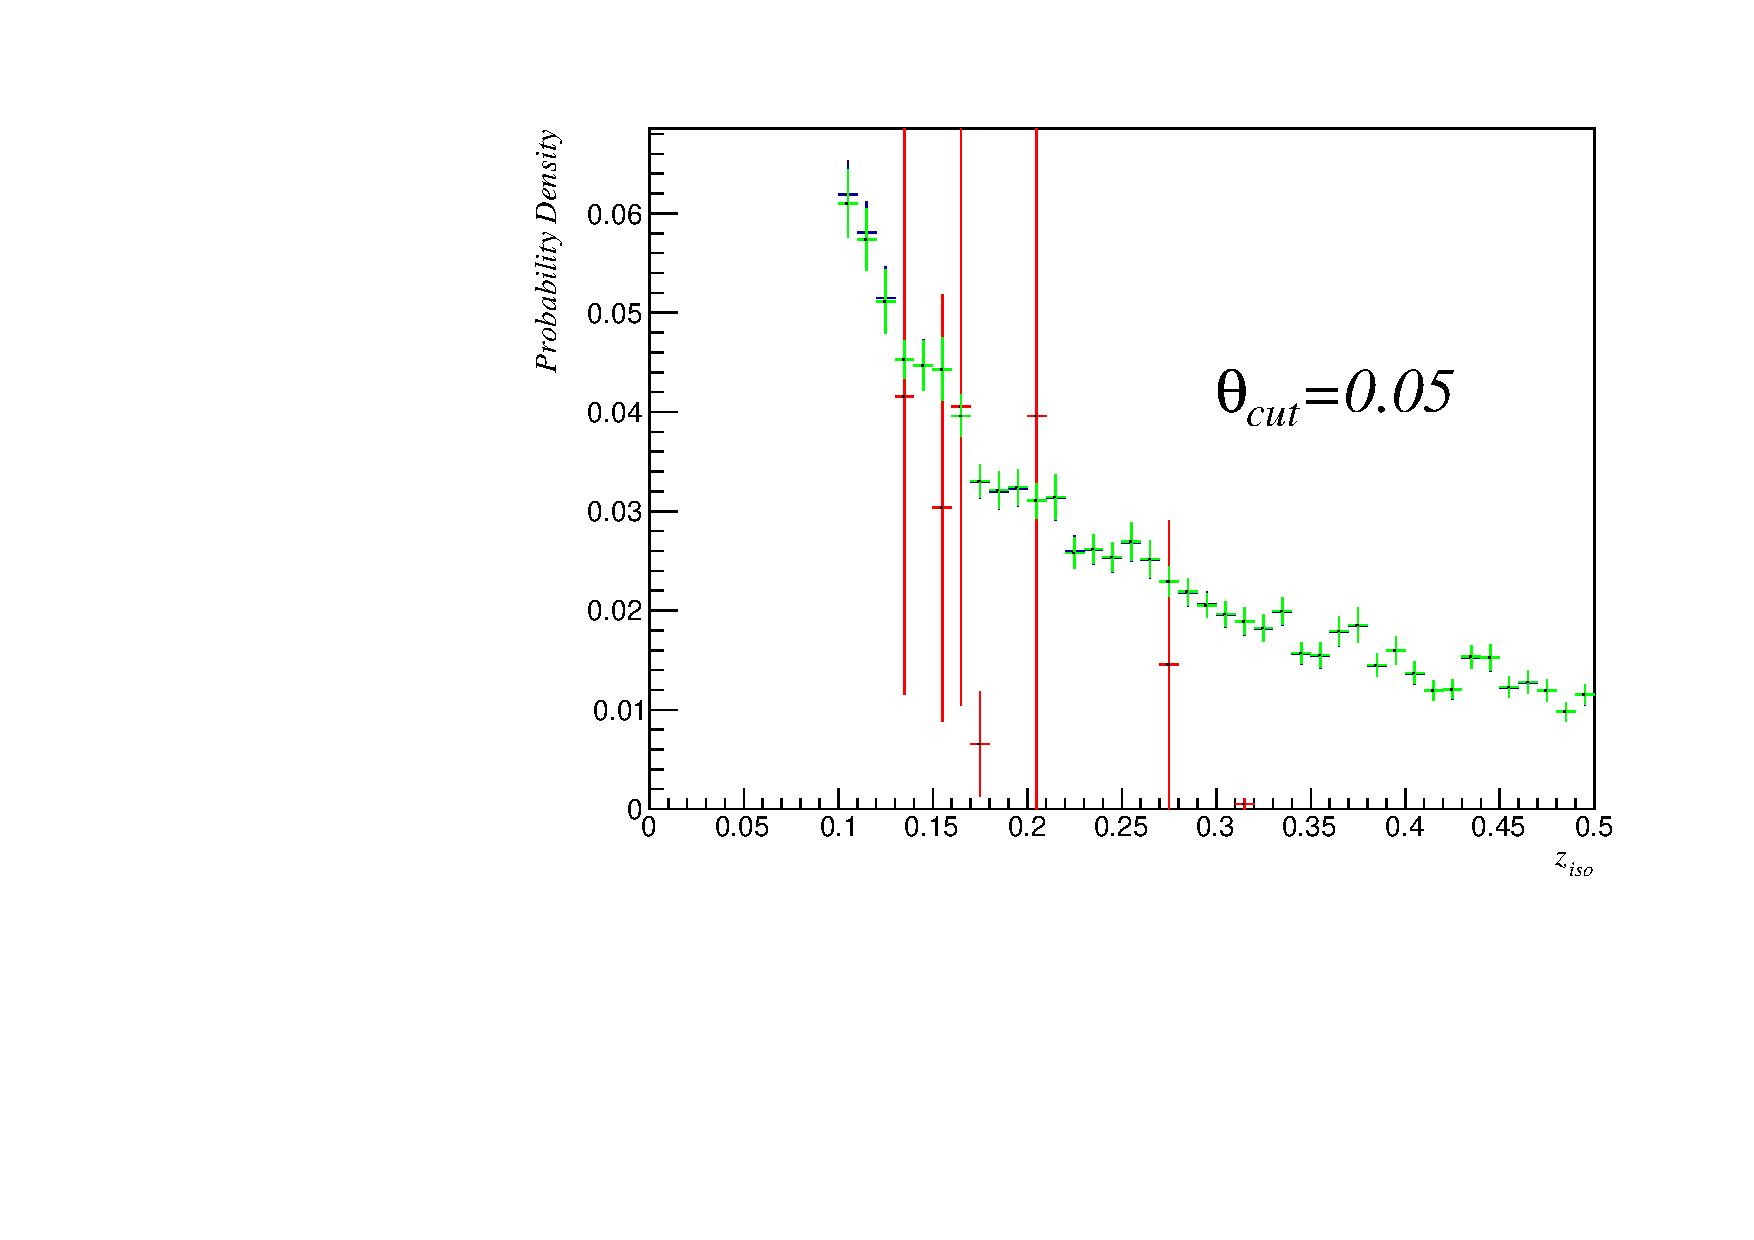
\includegraphics[width=\linewidth]{2.pdf}
				\caption{}
			\end{subfigure}
			\begin{subfigure}{0.47\textwidth}
				\centering
				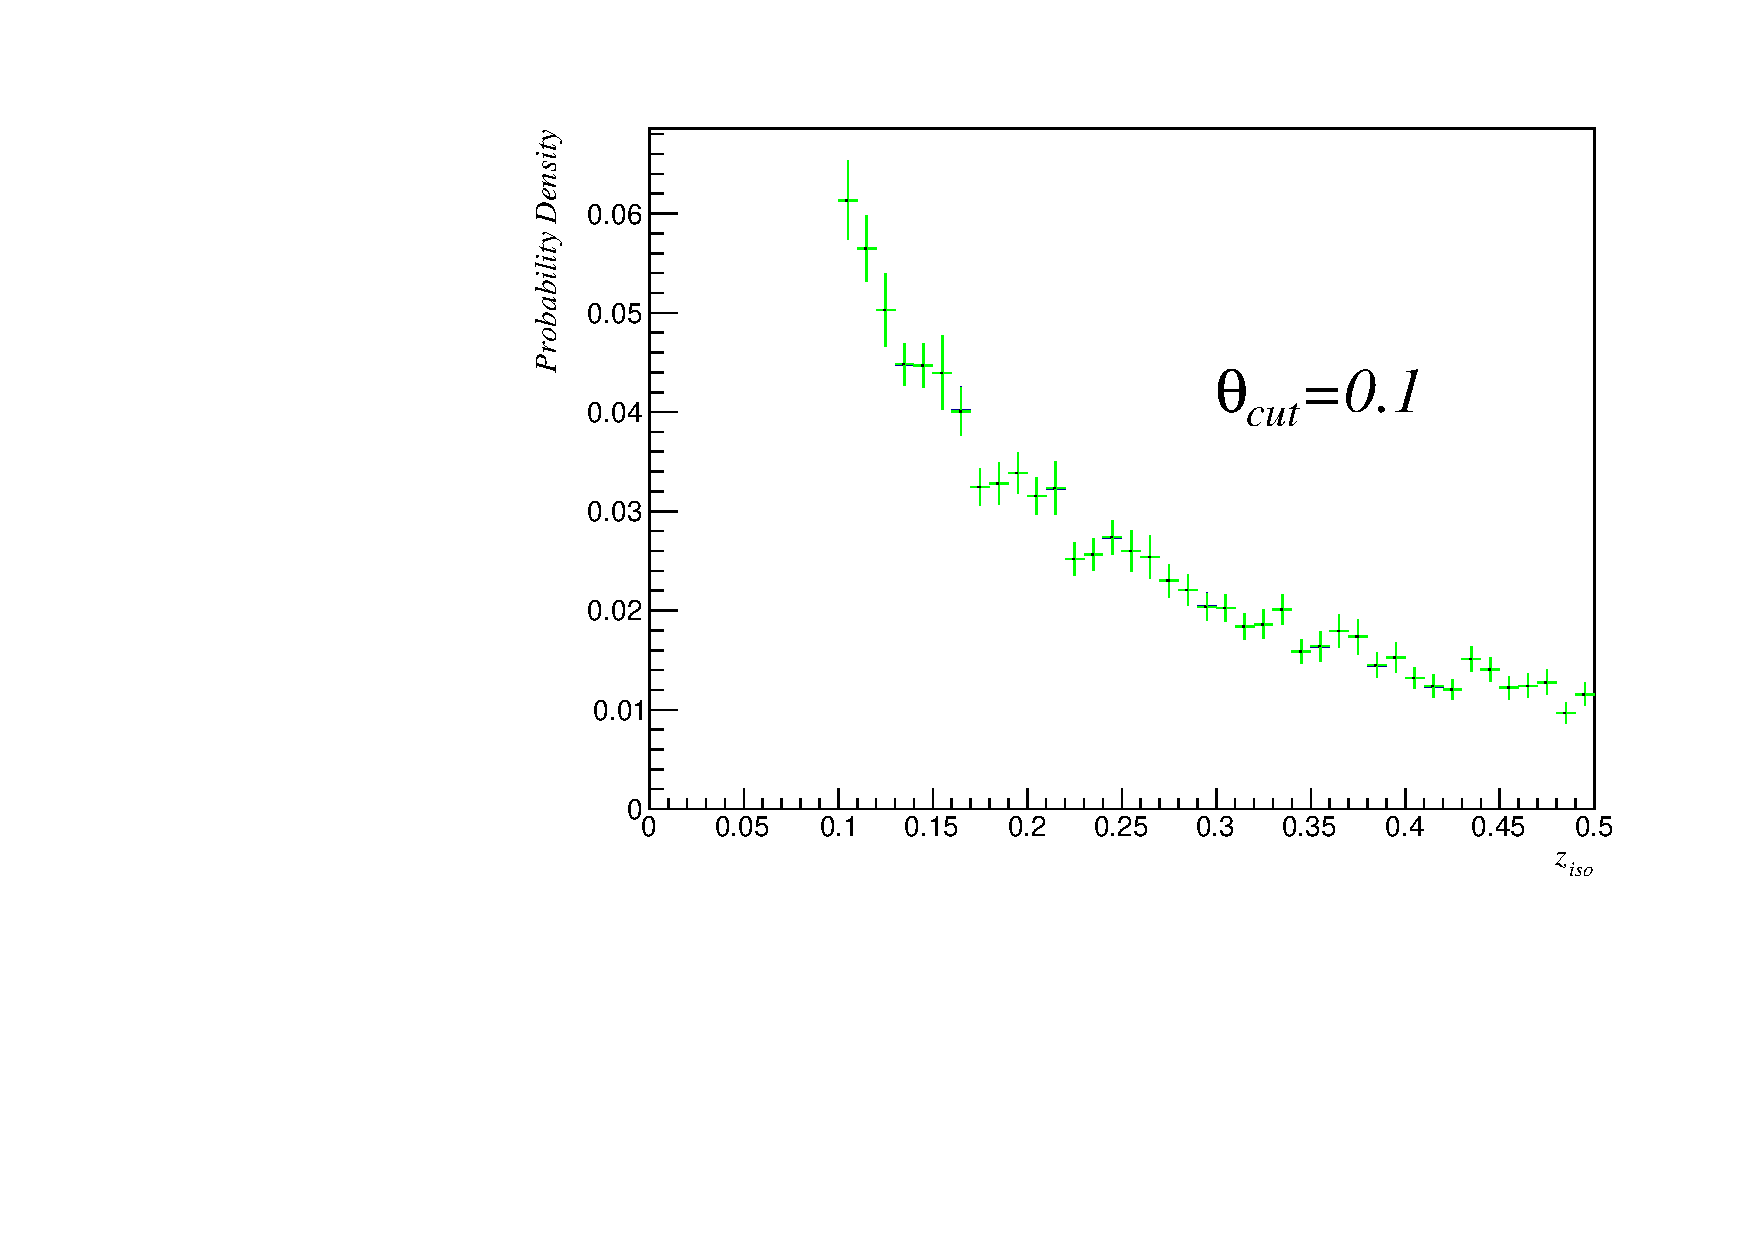
\includegraphics[width=\linewidth]{3.pdf}
				\caption{}
			\end{subfigure}
			\caption{$z$ distribution with $\theta_{\mathrm{cut}}$}
		\end{figure}
		In Fig. 3a, we set a $\theta_{\mathrm{cut}}$ to be 0.05, that is, only the splittings whose $\Delta R_{12}>\theta_{\mathrm{cut}}$
		are shown on the plot. Obviously many splittings from decay vanish. And when increase the $\theta_{\mathrm{cut}}$ to 0.1,
		there are no splittings from meson decay.\par
		The angular separation $\Delta R$ is used to identify and classify particles. A small $\Delta R$ indicates particles
		that are close together, possibly originating from a common parent. A larger $\Delta R$ suggests particles that are more
		widely separated, possibly from distinct origins. In the decay of mesons, which are composite particles formed by a quark
		and an antiquark bound together by the strong force, the close proximity of daughter particles arises from the fundamental
		characteristics of the strong force and the behavior of quarks. The strong force, acting over short ranges, binds quarks
		tightly, and the phenomenon of color confinement ensures that quarks are always found within bound states. When a meson
		undergoes decay, the quark and antiquark experience interactions dictated by the strong force, leading to daughter particles
		that are close together, which makes them have a small angular separation.\par
		\begin{wrapfigure}{l}{0.7\textwidth}
			\centering
			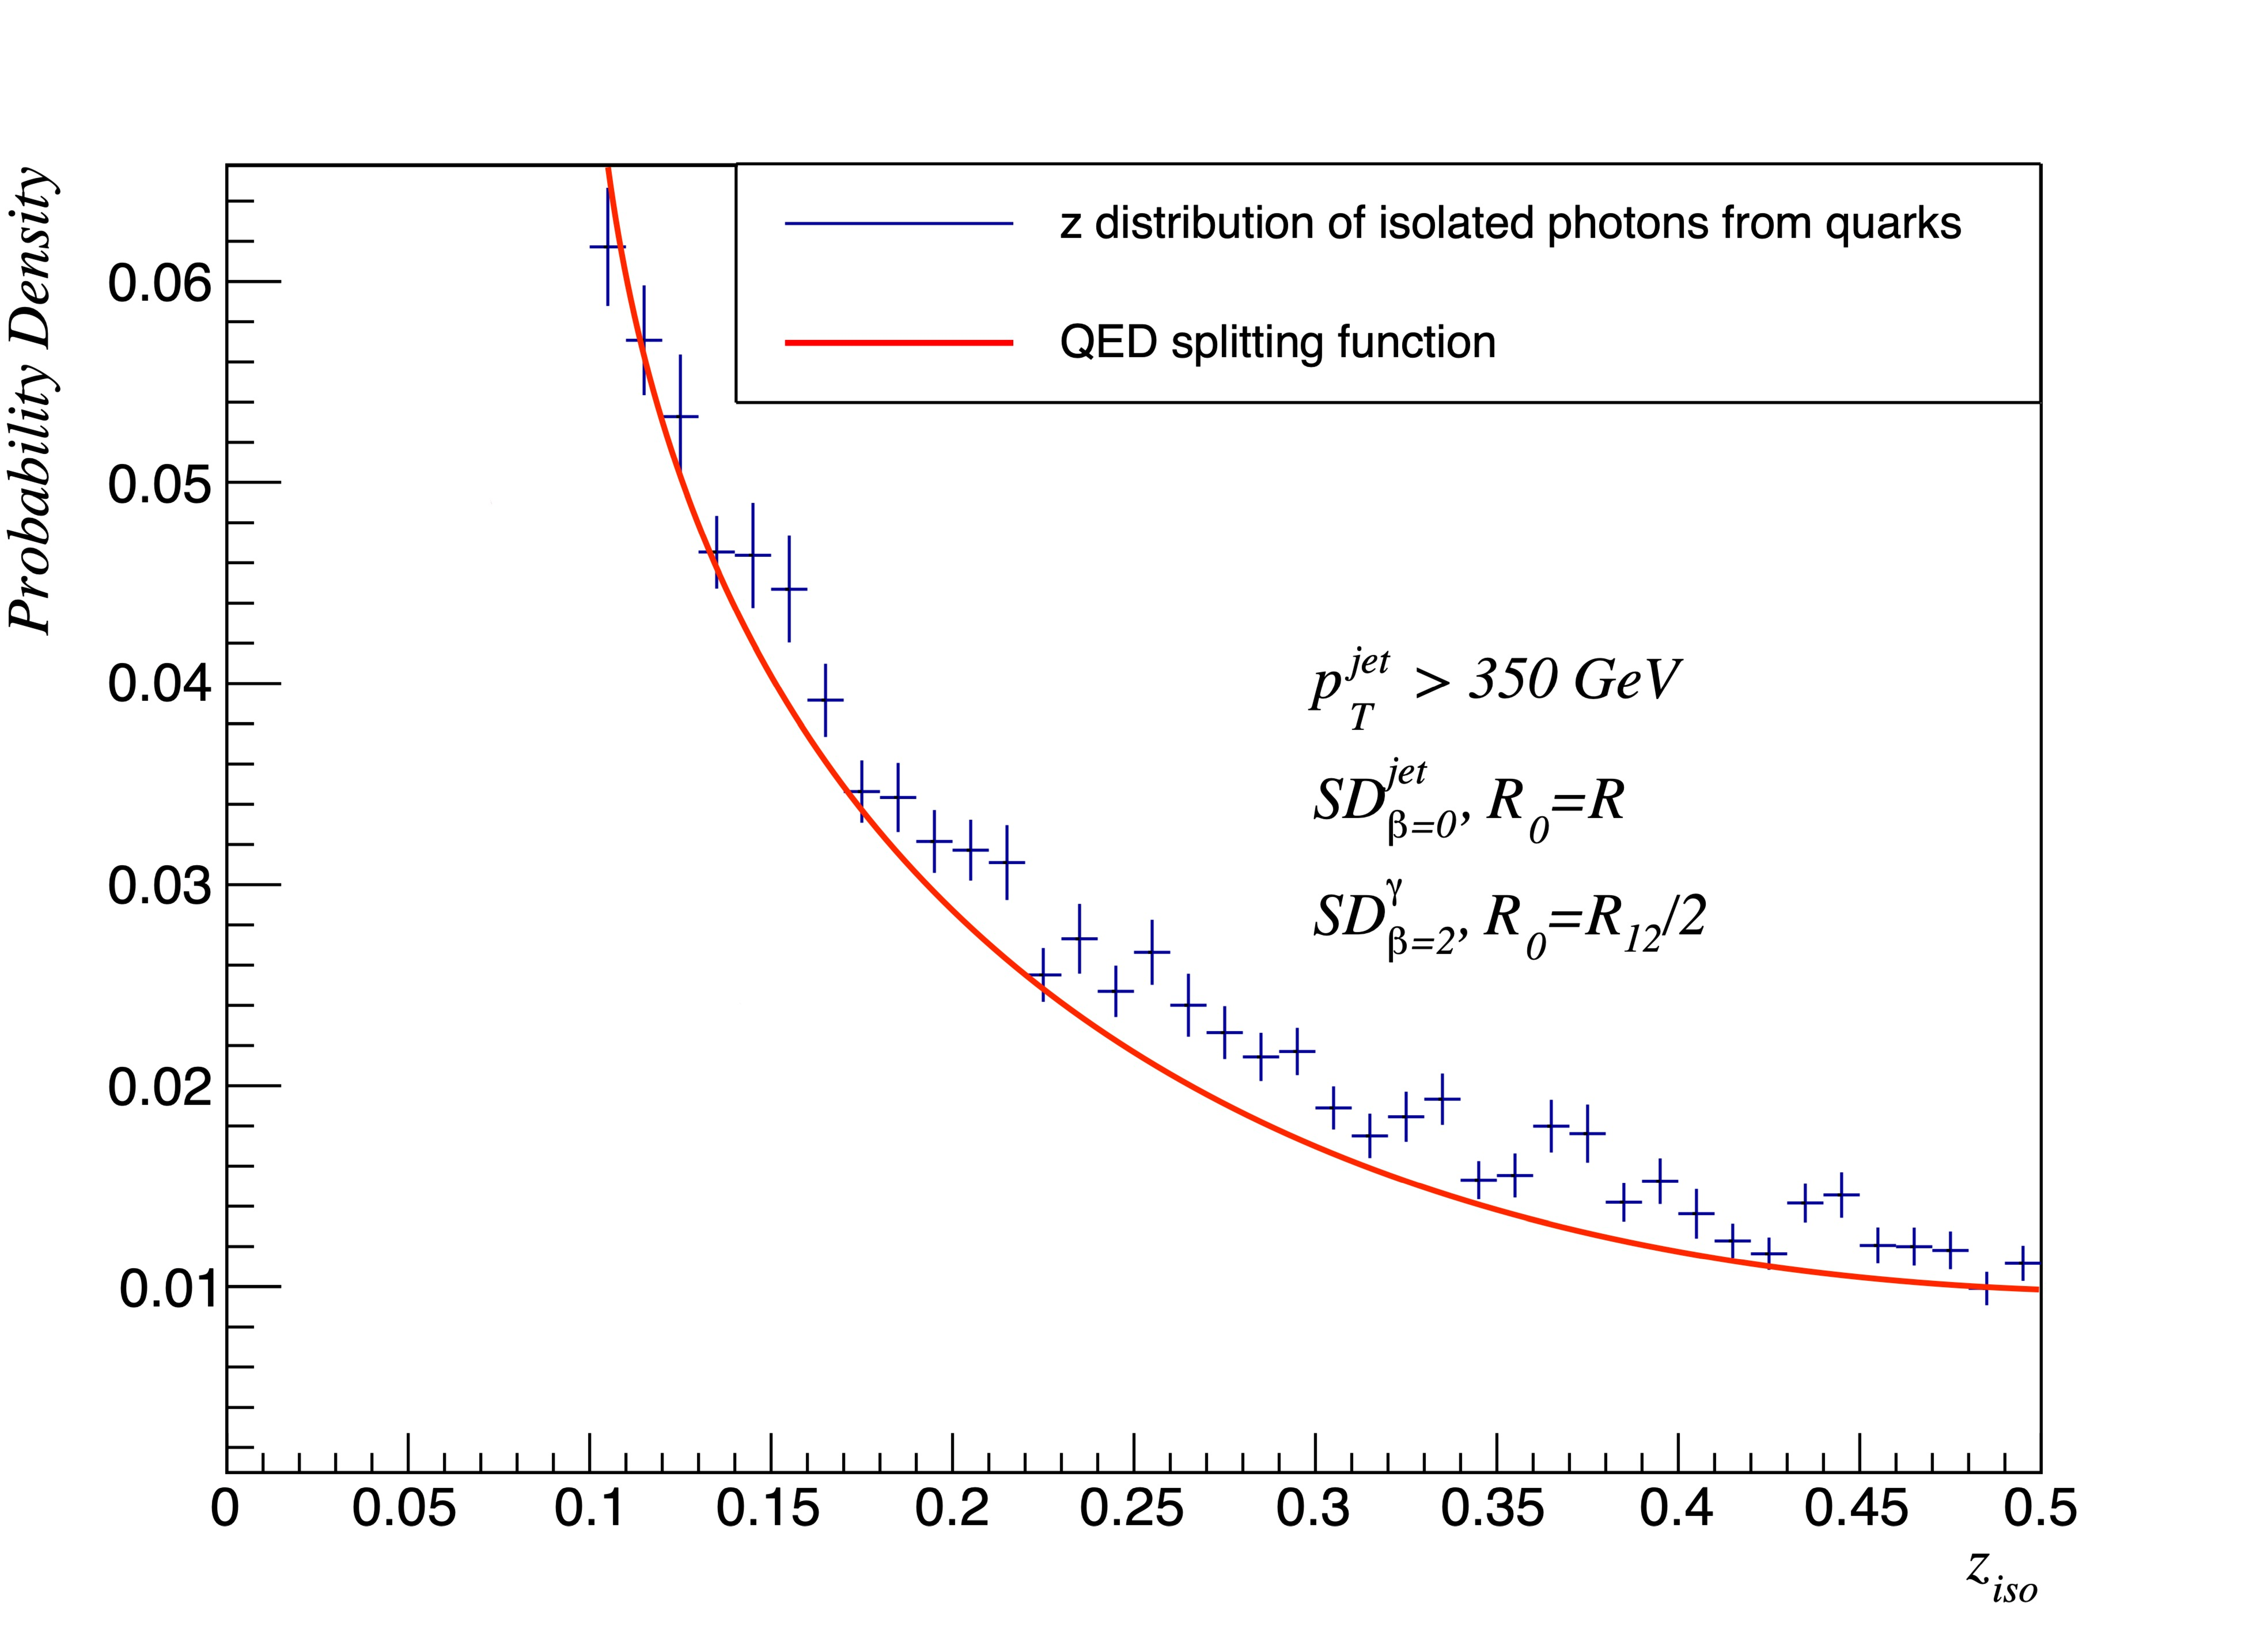
\includegraphics[width=\linewidth]{5.pdf}
			\caption{QED splitting function and isolated photons from quarks}
		\end{wrapfigure}
		Here in Fig. 4, we plot the QED splitting function with $z$ distribution of quark photons. The similarity in shape between
		the QED splitting function and the $z$ distribution of quark photons in the plot suggests a correlation between the
		probability distribution of momentum sharing (described by the QED splitting function) and the actual observed momentum
		distribution (represented by the $z$ values). This correlation indicates that the characteristics of photon emissions
		in the quark-to-photon process (such as how the momentum is shared between the quark and the emitted photon) are in line
		with the theoretical expectations set by Quantum Electrodynamics (QED). This congruence is crucial for validating the
		theoretical framework and enhances our understanding of the underlying physics in high-energy processes involving quarks
		and photons.

\section{Acknowledgments}
	I thank Prof. Leticia Cunqueiro, it was her who offered me an opportunity to learn about high-energy experiment from scratch.
	Her patient encouragement and guidance have been invaluable throughout this endeavor. I am truly appreciative of the
	knowledge and skills I have gained under her mentorship. I also thank Dr. Cristian Baldenegro, Dr. Jelena Mijuskovic and 
	Dr. Vangelis Valdimirov. They have been not only great colleagues but also friends and mentors, and I appreciate their assistance
	in both my academic and personal journey.\par
	This work was supported by the Pilot Scheme of Talent Training in Basic Sciences (Boling Class of Physics, Nankai University), Ministry of Education.

\bibliographystyle{unsrt}
\bibliography{example}
\end{document}